\section{Funktionsweise der Werkzeuge}

Dieses Kapitel wird sich mit der internen Funktionsweise der gebräuchlichsten statischen Code Analyse Tools für Java beschäftigen. Diese sind wie in vorherigen Kapiteln dargestellt: Findbugs, Checkstyle, PMD sowie Emma, welches den Code zwar nicht statisch analysiert, im Rahmen der Vorlesung aber trotzdem im Context der statischen Analyse besprochen wurde.


\subsection{FindBugs}

FindBugs ist ein von der Universität von Maryland initiiertes Software-Projekt zur statischen Code Analyse. FindBugs genießt große Verbreitung in der Industrie und wird von Firmen wie Google und ehemals Sun Microsystems nun Oracle unterstüzt.
FindBugs arbeitet vollständig auf dem Java-Bytecode und kann dadurch auch auf "binären" Projektdistributionen durchgeführt werden. 

FindBugs bietet eine große Anzahl an mitgelieferten Fehler-Pattern, die in verschiedene Warnstufen eingeteilt sind. Ihr Hauptfokus liegt auf der Erkennung von fehlerhaftem Code, der bei der Ausführung zu Runtime-Fehlern führen würde.

Möchte man seine eigenen Fehler-Pattern hinzufügen, bietet Findbugs dafür ein Plugin Konzept, welches allerdings ein Verständnis der internen Funktionsweise von FindBugs voraussetzt.
 
FindBugs nutzt für die ByteCode Analyse die Apache BCEL Library, welche eine gut nutzbare Schnitstelle zu komplierten Java Class Files bietet, welche in vielen Bytecode-nahen Projekten eingesetzt wird.

Dies kann für Entwickler einen großen Nachteil bedeuten, da die wenigstens ein Verständnis von ByteCode haben. Man muss beachten, dass die baumartige Struktur des Sourcecodes im Bytecode, wie auch in Maschinensprache, zu einer flachen sequenziellen Abfolge von Instruktionen wird. 

Weiter erschwert das Erstellen eines eigenen Fehler-Pattern, dass der Bytecode sequenziell Durchlaufen wird und der Bytecode Scanner dabei bei jeder Instruktion die ihm zugeordnenten Fehler-Detectoren über ein Visitor-Pattern aufruft. 
Dadurch ist der Entwickler des Fehler-Detektor dafür verantwortlich, sich die bereits gescannten Instruktionen in seinem State zu speichern. Hierfür bietet sich i.d.R. eine Statemaschine an. Aber auch dies ist ein Programmierparadigma, das bei vielen Entwicklern in Zeiten von OOP nicht mehr häufig genutzt wird und somit eine weitere Hürde in der Erstellung von eingenen Fehler-Mustern darstellt.

Die Analyse des Bytecodes hat aber auch positive Seiten. So ist zum einen die Analyse sehr perfomant, da sie einfach einer linearen Abarbeitung von Instruktionen entspricht und zum anderen ist die der Bytecode bereits durch den Java Compiler optimiert worden und somit verringert sich die Häufigkeit eines False-Positives.

In der Usability bietet FindBugs auch Vorteile gegenüber anderen Tools. So bietet es zum einen eine sehr gute und aktuelle Integration in viele Eclipse und viele andere Entwicklungsumgebungen und lässt sich zum anderen über ein Konsolen-Tool einfach in automatische Build-Prozesse einbinden.


\subsection{PMD}
PMD, dessen Name nach eigenen Aussagen des Projekts keine ausgeschriebe Bedeutung hat, ist ebenfalls ein Werkzeug zur statischen Code Analyse von Java-Code. 

PMD liefert ebenfalls eine Vielzahl an eingebauten Regeln, die anders als bei FindBugs nicht so sehr auf potentielle Fehler, sondern eher auf ineffizenten Code ausgelegt sind. Beispiele hierfür sind z.B. leere Blöcke, toter Code oder die falsche Verwendung von Strings und StringBuffern. 

PMD besitzt weiter einen Copy/Paste Detector, der es erlaubt, mit des Rabin-Karp-Algorithmuses duplizierten Code zu finden.

PMD operiert, anders als FindBugs, nicht auf den binären Java Class Files, sondern auf dem Source-Code. Genauer gesagt, auf dem Abstract Syntax Tree, der aus dem Source-Code vor dem Erstellen des Bytecodes erzeugt wird. 

Die Analyse des ASTs ist zwar nich so performant, wie das einfache Scannen von Bytecode, besitzt für das Entwicklen von eigenen Regeln aufgrund der Nähe zum Sourcecode aber entsprechende Vorteile.

Bei der Transformation von Quelltext zu einem Abstract Syntax Tree gehen (im Gegensatz zu Bytecode) keine Informationen über die Struktur des Quelltextes verloren. Es wird einzig der vorhandene Quelltext in einem Baum abgebildet. 
Möchte man nun seine eigenen PMD Regeln hinzufügen, reicht es aus den AST zu travasieren und auf das Vorkommen des entsprechenden Musters zu untersuchen. PMD bietet für diese Aufgabe ein eigenes Entwicklungstool an, dass den erzeugten AST darstellt, und in dem man explorativ dieses Baum travasieren kann.

\begin{figure}[htbp]
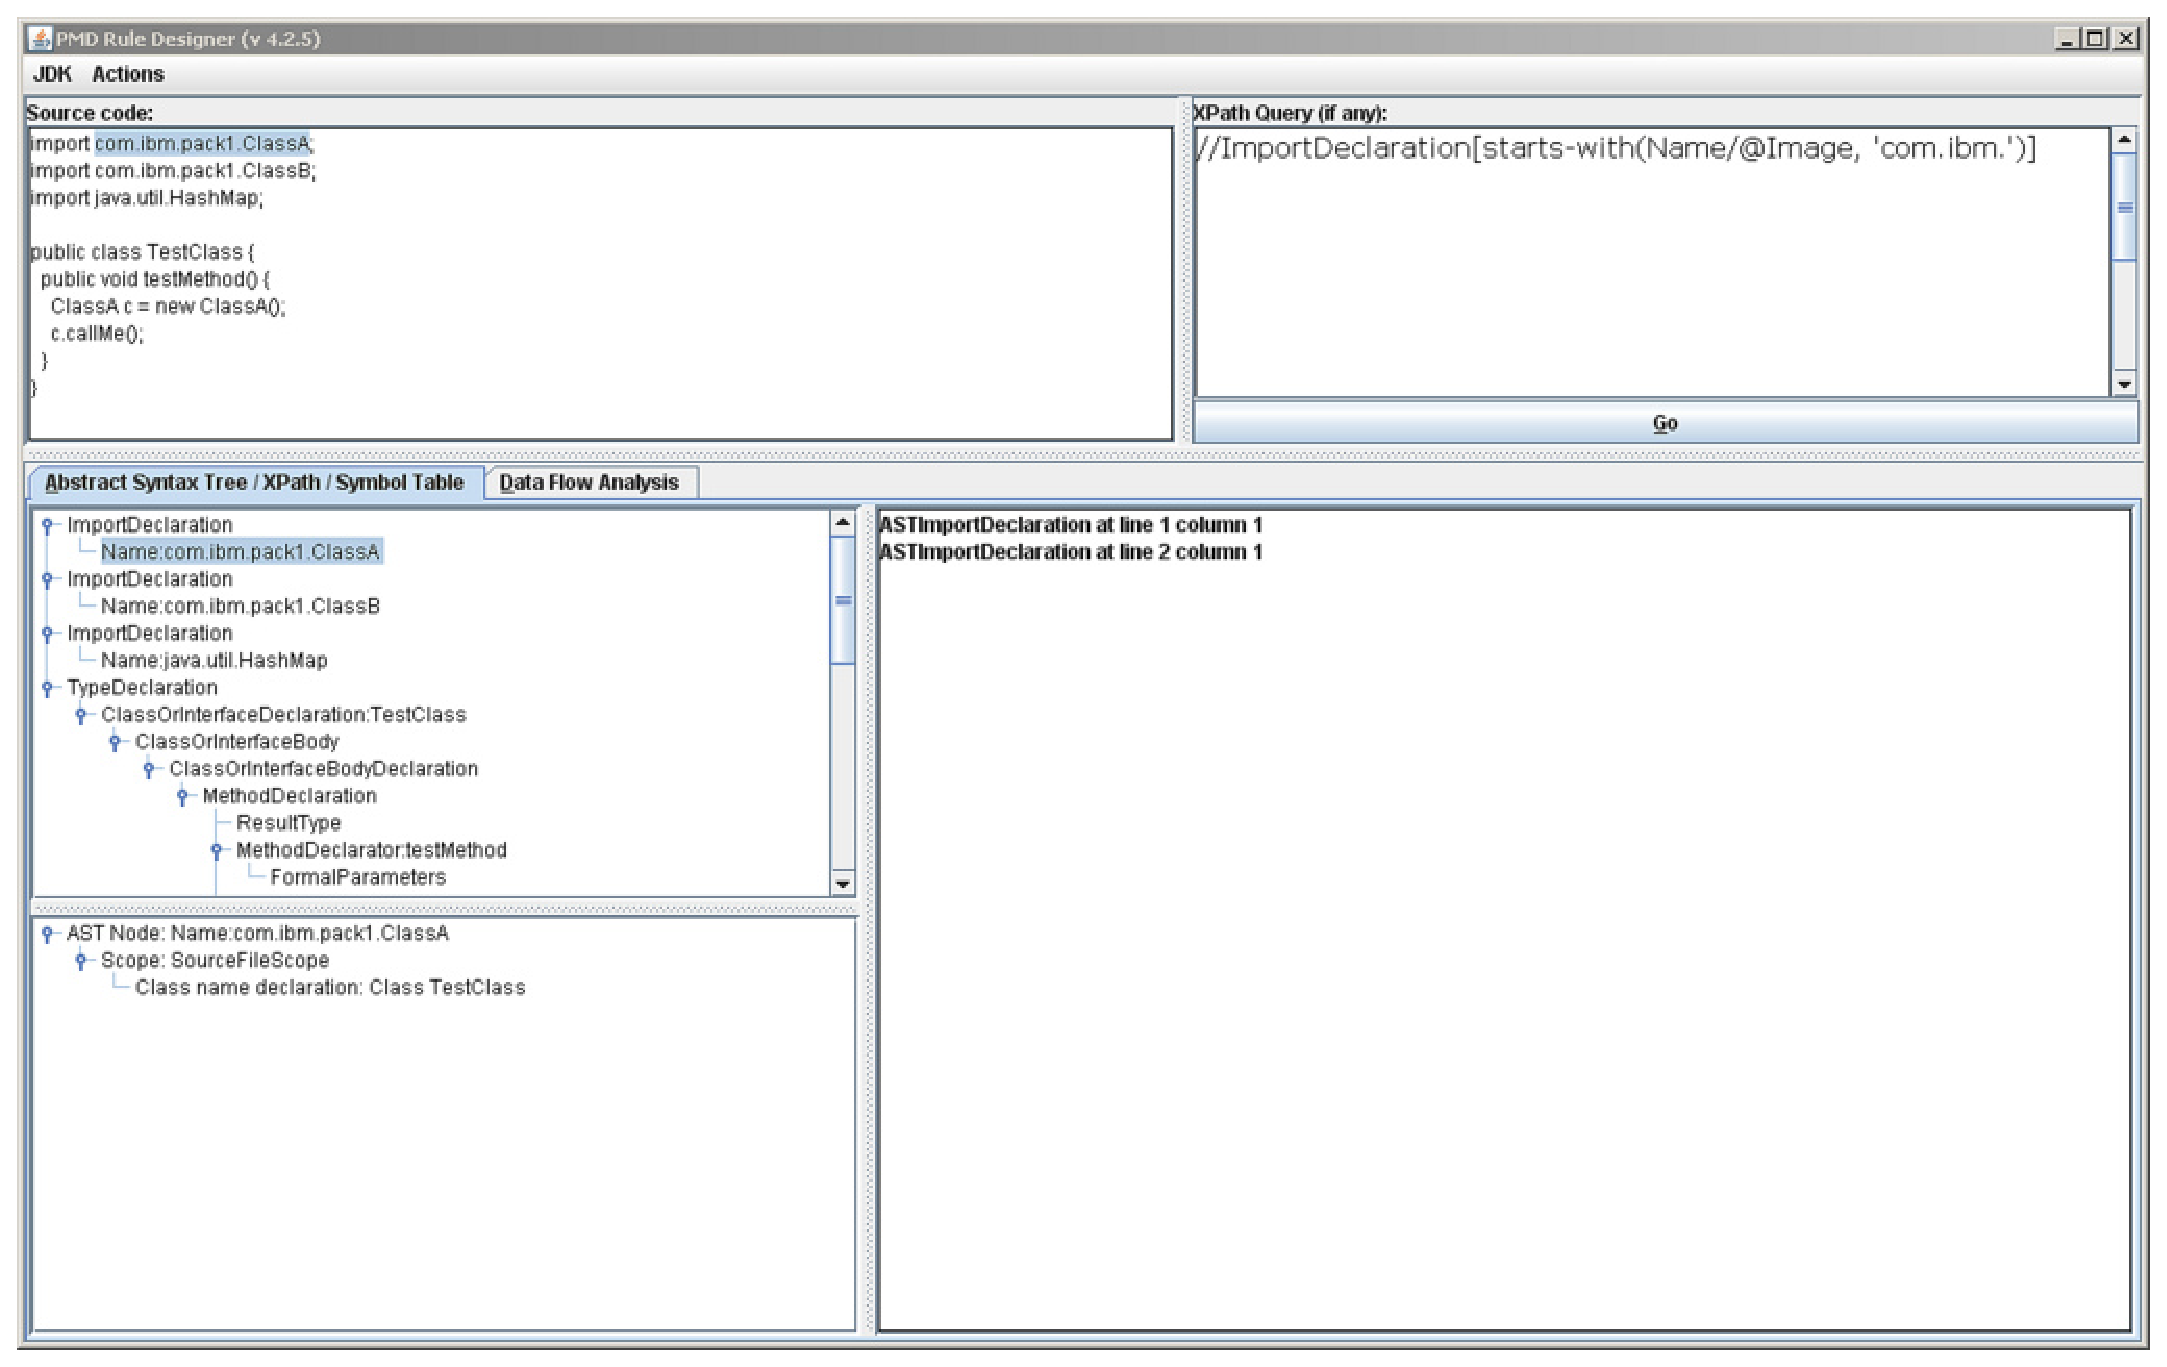
\includegraphics[width=10cm]{pmd-dev}
\caption{PMD Entwicklungs Werkzeug}
\end{figure}

Die Analyse auf einem AST bietet einen weiteren Vorteil. Da Bäume eine weit verbreitete Darstellungsform sind, gibt es bereits eine vielzahl von Werkzeugen die auf Ihnen operrieren können. Das in diesem Kontext wichtigste ist XPath.

PMD bietet neben der Schnitstelle für in Java implementierte Regeln, ebenfalls eine Schnittstelle für XPath. 

XPath oder auch XML Path Language ist eine vom W3-Konsortium entwickelte Abfragesprache, um Teile eines XML-Dokumentes (welches ebenfalls Bäume sind) abzufragen. Dabei bietet es eine sehr einfache Möglichkeit, Bäume zu travasieren.

\begin{lstlisting}
//child:Buch[count(./Seite)<=100]
/count(.Seite)>=10]
\end{lstlisting}

Das Beispiel würde z.B. alle Bücher aus einem Baum liefern, das maximal 100 doch mindestens 10 Kindelemente/Seiten hat.

Diese XPath-Ausdrücke können direkt in den PMD-Konfigurations-Files angegeben werden und machen es so für einfache und mittel komplexe Regeln überflüssig, eigene Java-Module zu implementieren.

PMD besitzt ebenfalls ein Konsolen-Tool, das sich sehr gut in den Build-Prozess integrieren lässt. Das entsprechende Eclipse Plugin ist zum Zeitpunkt dieses Papers leider nicht auf dem aktuellsten Stand und nutzt noch PMD Version 4, welche zur Version 5 inkompatibele Konfigurations-Dateien besitzt. Soll also die aktuellste PMD Version 5 im Build-Prozess verwendet werden, müssen zwei Konfigurations-Dateien für Version 4 und 5 gepflegt werden.


\subsection{Checkstyle}

Checkstyle ist das dritte wichtige statische Code Analyse Tool in der Java-Welt. Der Fokus von Checkstyle liegt weder in der effizenten Nutzung der JVM noch in dem Auffinden von Programmierfehlern, sondern vor allem in der Prüfung eines einheitlichen Programmierstils. 
Dafür liefert Checkstyle viele Regeln von Haus aus mit, die in Form von Modulen gruppiert sind. Einige Beispiele an mitgliefierten Modulen sind:
\begin{itemize}
\item Class Design, welches Prüfungen zum Softwaredesign beinhaltet
\item Coding, welches allgemeine Codingguidelines pürft.
\item Javadoc Comments zum Prüfen der Vollständigkeit und der richtigen Formatierung von Javadoc-Kommentaren
\item Metrics zur Einhaltung diverser Sofwaremetriken
\item Naming Convetions, um die Einhaltung von Namenskonventionen zu prüfen
\item Whitspaces zur Prüfung des Quelltextes hinsichtlich Leerzeichen und korrekter Einrückung.
\end{itemize}
Checksyle arbeitet ähnlich wie PMD auf dem AST und kann durch eigene Java-Module, die ebenfalls auf dem AST arbeiten, erweitert werden. Checkstyle bietet zur Erweierung noch eine weitere sehr nützliche Schnitstelle. So bietet das Modul 'Regexp' es dem Entwickler an, eigene Regeln mithilfe von regulären Ausdrücken zu schreiben. Dies dürfte gerade beim Überprüfen von Codeguildelines oft als ausreichend empfunden werden und bietet eine sehr einfache Schnitstelle, um Checkstyle zu erweitern.

Checkstyle lässt sich wie PMD und FindBugs sehr einfach über ein Konsolen-Werkzeug in den Build-Prozess einbinden und bietet ein gut funktionierendes Eclipse-Plugin.


\subsection{Emma}

Emma ist eine Code Coverage Library von Vlad Roubtsov. Sie zählt eigentlich nicht zu den statischen Code Analyse Tools, soll aber, da sie im Rahmen der Vorlesung im Kontext solcher behandelt wurde, hier kurz erläutert und zur statischen Code Analyse abgegrenzt werden. 
Das Ziel von Emma ist zu analysieren, welcher Code durchlaufen wird. Diese Information ist zum Beispiel für die Ermittlung einer Testabdeckung sehr interessant. Emma untersützt dabei eine Vielzahl von Metriken, die aber in den entsprechenden Ausarbeitungen zum Thema Testabdeckung zu finden sind. In diesem Kontext soll nun auf die Funktionsweise von Emma eingegangen werden.

Wie bereits erwähnt, ist Emma kein Werkzeug der statischen Code-Analyse. Die Funktionsweise von Emma basiert auf der Instrumentierung von Java Bytecode. Dazu untersützt Emma zwei Verfahren. Zum einen kann in einem zweiten "compile" Schritt der Bytecode um entsprechende Hooks erweitert werden, die dem Emma Toolkit die nötigen Daten über den durchlaufenden Code geben, und zum Anderen kann die Applikation mit einem speziellen Emma-Classloader gestartet werden, der den geladenen Bytecode on-the-fly instrumentiert. Als nächstes wird ein Driver benötigt, der den Instrumentierten Code durchläuft. Dies kann sowohl durc ein manuelles bedienen der Applikation geschehen, als auch durch automatische Tests. Der am weitestverbreiteste Anwendungsfall ist wohl die bereits erwähnte Testabdeckung bei Unit-Tests. Aber als reines Code Coverage Tool ist Emma natürlich wesentlich vielseitiger. So kann ein weiterer Interessanter Ansatz sein, dass man sich in (geerbtem) Spagetthi-Code einen schnellen Überblick verschaffen will, welcher Code bei einer Benutzeraktion durchlaufen wird.

Emma lässt sich über Ant und Maven Plugins gut in den BuildProzess inegrieren und bietet gerade für den Fall der Testabdeckung mit EclEmma ein sehr gutes Eclipse Plugin.

